\section{How do generative models work? How do GANs compare to others?}
\label{sec:tree}

We now have some idea of what generative models can do and why it might be
desirable to build one.
Now we can ask: how does a generative model actually work? And in particular,
how does a GAN work, in comparison to other generative models?

To simplify the discussion somewhat, we will focus on generative models
that work via the principle of {\em maximum likelihood}.
Not every generative model uses maximum likelihood.
Some generative models do not use maximum likelihood by default, but
can be made to do so (GANs fall into this category).
By ignoring those models that do not use maximum likelihood, and
by focusing on the maximum likelihood version of models that do not
usually use maximum likelihood, we can eliminate some of the more 
distracting differences between different models.

The basic idea of maximum likelihood is to define a model that provides
an estimate of a probability distribution, parameterized by parameters
$\vtheta$.
We then refer to the {\em likelihood} as the probability that the model
assigns to the training data: $\prod_{i=1}^m \pmodel\left(\vx^{(i)}; \vtheta \right),$
for a dataset containing $m$ training examples $\vx^{(i)}$.

The principle of maximum likelihood simply says to choose the parameters for the model
that maximize the likelihood of the training data.
This is easiest to do in log space, where we have a sum rather than a product
over examples.
This sum simplifies the algebraic expressions for the derivatives of the likelihood
with respect to the models, and when implemented on a digital computer, is less
prone to numerical problems, such as underflow resulting from multiplying together
several very small probabilities.

\begin{align}
\vtheta^* =& \argmax_\vtheta \prod_{i=1}^m \pmodel\left(\vx^{(i)}; \vtheta \right) \\
  =& \argmax_\vtheta \log \prod_{i=1}&m \pmodel\left(\vx^{(i)}; \vtheta \right) \label{eq:log} \\
          =& \argmax_\vtheta \sum_{i=1}^m \log \pmodel\left(\vx^{(i)}; \vtheta \right).
\end{align}

In \eqref{eq:log}, we have used the property that $\argmax_v f(v) = \argmax_v \log f(v)$ for 
positive $v$, because the logarithm is a function that increases everywhere and does not change
the location of the maximum.

The maximum likelihood process is illustrated in \figref{fig:mle}.

We can also think of maximum likelihood estimation as minimizing the
{\em KL divergence} between the data generating distribution and the
model:
\[ \vtheta^* = \argmin_\vtheta \KL\left( \pdata(\vx) \Vert \pmodel(\vx ; \vtheta) \right). \]
If we were able to do this precisely, then if $\pdata$ lies within the family of distributions
$\pmodel(\vx ; \vtheta)$, the model would recover $\pdata$ exactly.
In practice, we do not have access to $\pdata$ itself, but only to a training set
consisting of $m$ samples from $\pdata$.
We uses these to define $\ptrain$, an {\em empirical distribution} that places mass only
on exactly those $m$ points, approximating $\pdata$.
Minimizing the KL divergence between $\ptrain$ and $\pmodel$ is exactly equivalent to maximizing
the log-likelihood of the training set.

\begin{figure}
\centering
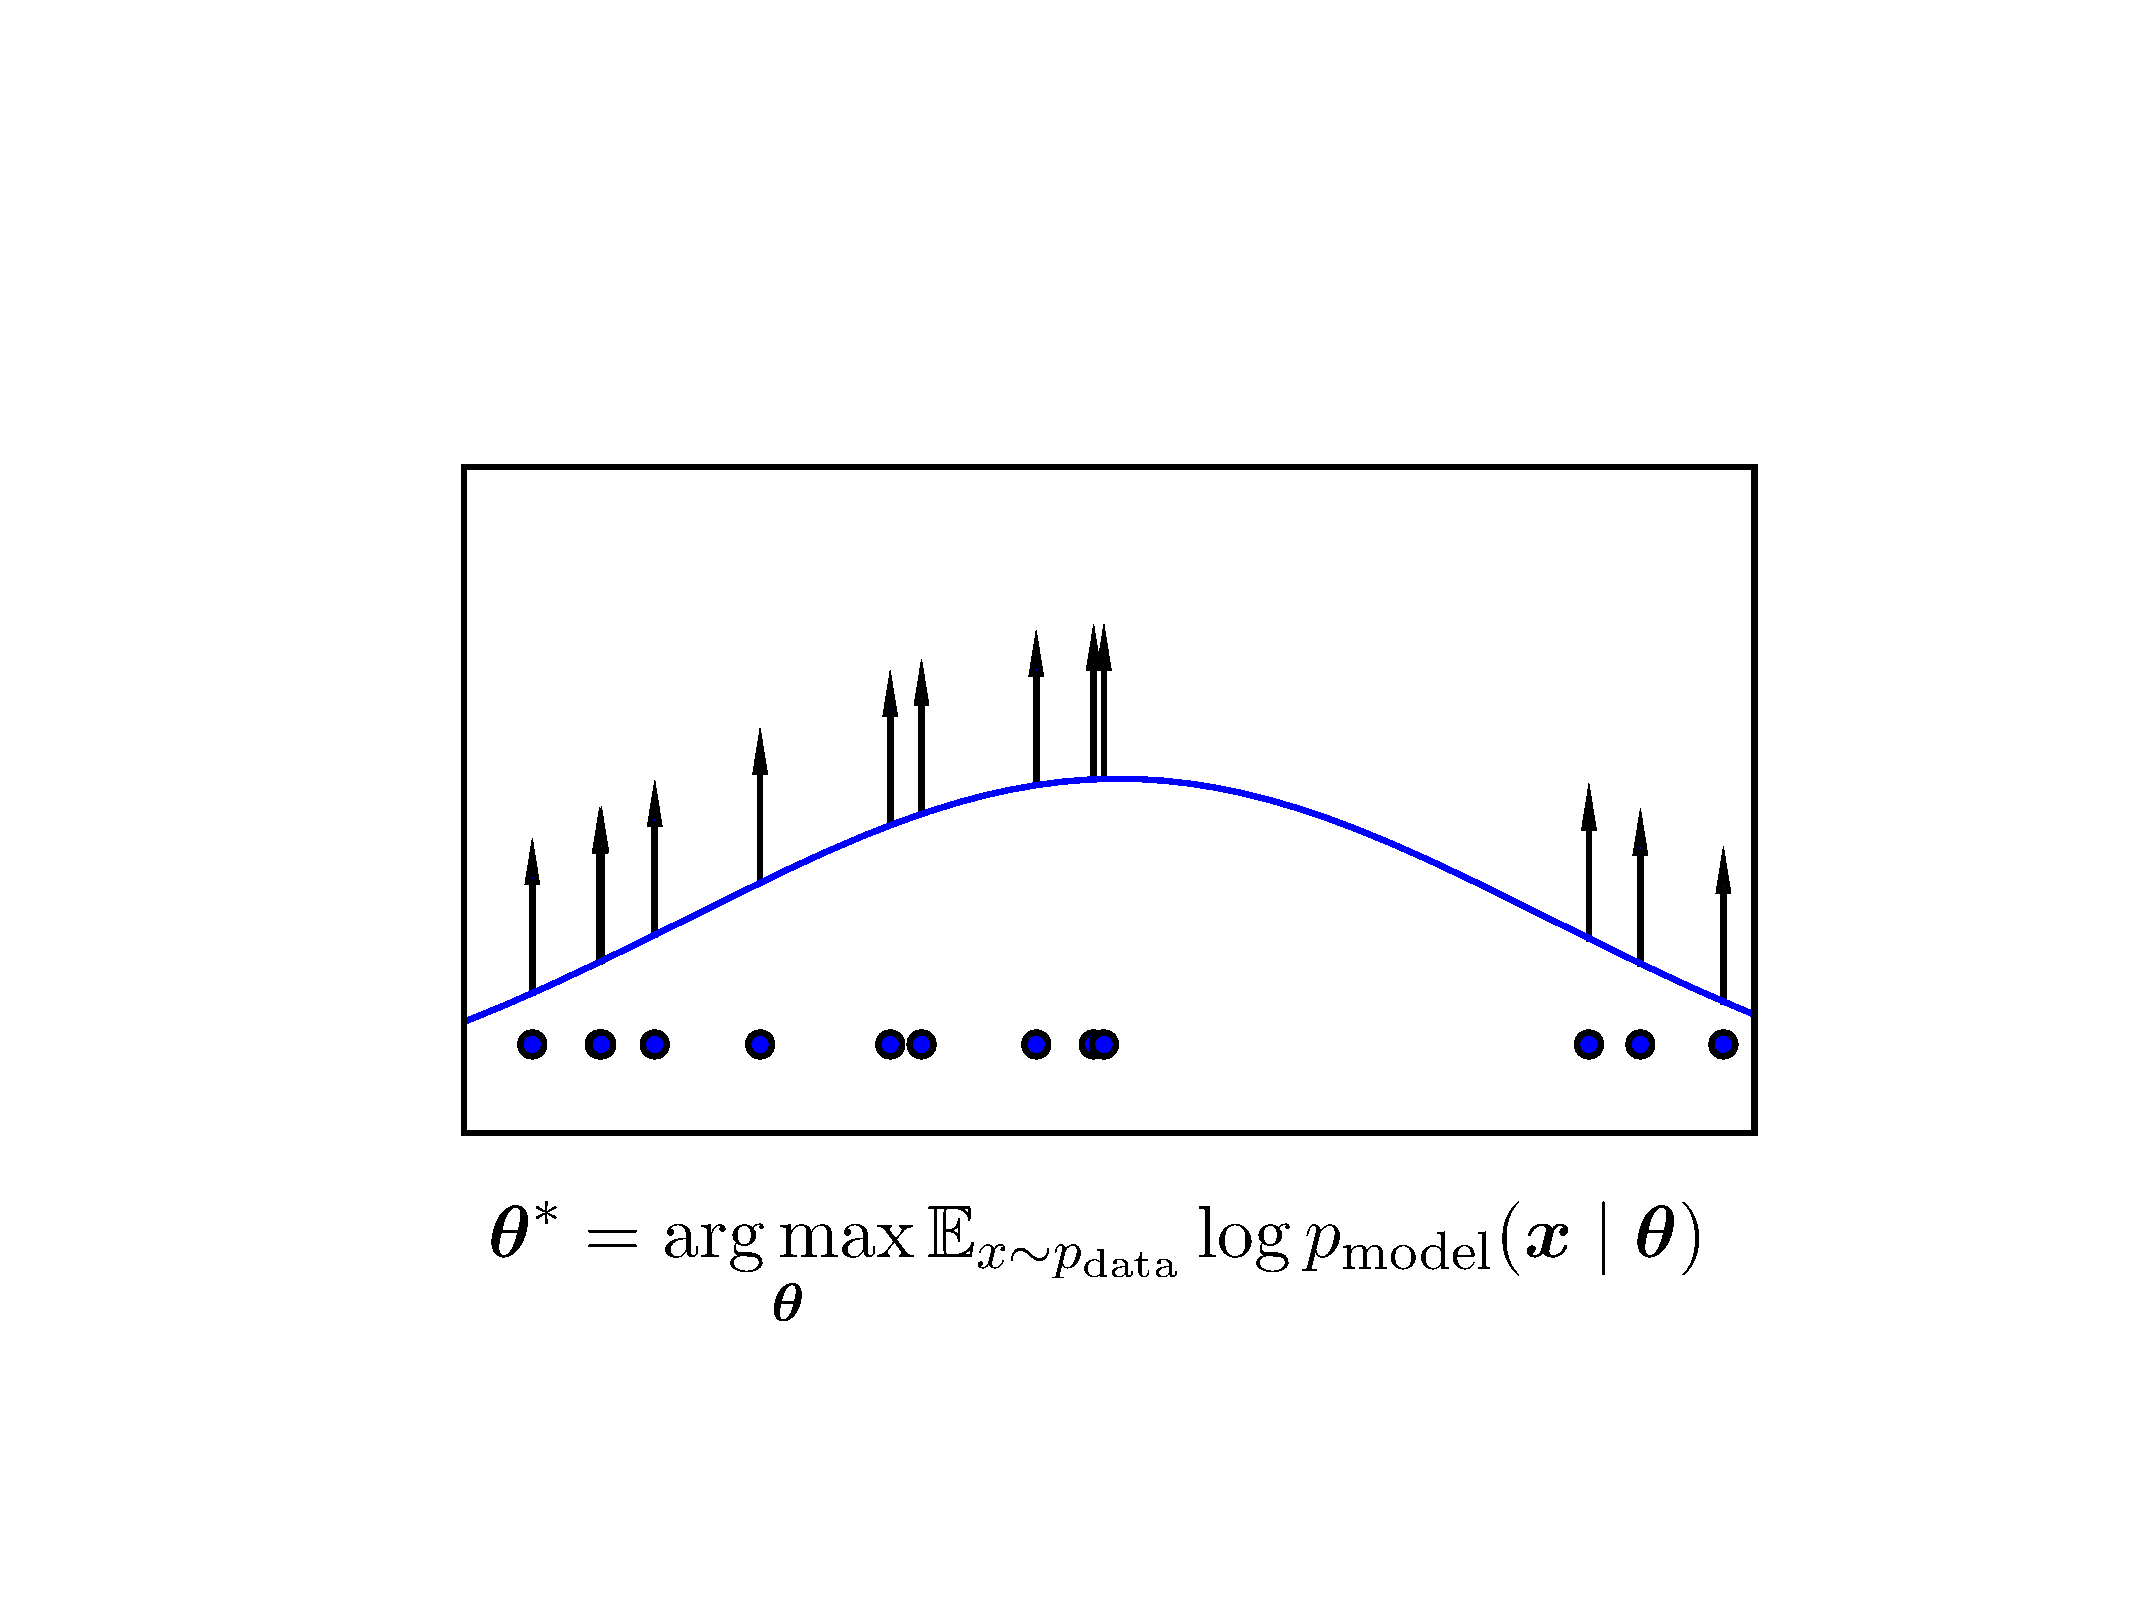
\includegraphics[width=\textwidth]{mle.pdf}
\caption{The maximum likelihood process consists of taking several samples from
  the data generating distribution to form a training set, then pushing up on the
  probability the model assigns to those points, in order to maximize the likelihood
  of the training data.
  This illustration shows how different data points push up on different parts of
  the density function for a Gaussian model applied to 1-D data.
  The fact that the density function must sum to $1$ means that we cannot simply
  assign infinite likelihood to all points; as one point pushes up in one place
  it inevitably pulls down in other places.
  The resulting density function balances out the upward forces from all the data
  points in different locations.
}
\label{fig:mle}
\end{figure}


\subsection{A taxonomy of deep generative models}

If we restrict our attention to deep generative models that work by maximizing
the likelihood, we can compare several models by contrasting the ways that they
compute either the likelihood and its gradients, or approximations to these
quantities.
As mentioned earlier, many of these models are often used with principles other
than maximum likelihood, but we can examine the maximum likelihood variant of
each of them in order to reduce the amount of distracting differences between
the methods.
Following this approach, we construct the taxonomy shown in \figref{fig:tree}.
Every leaf in this taxonomic tree has some advantages and disadvantages.
GANs were designed to avoid many of the disadvantages present in pre-existing
nodes of the tree, but also introduced some new disadvantages.

\begin{figure}
\centering
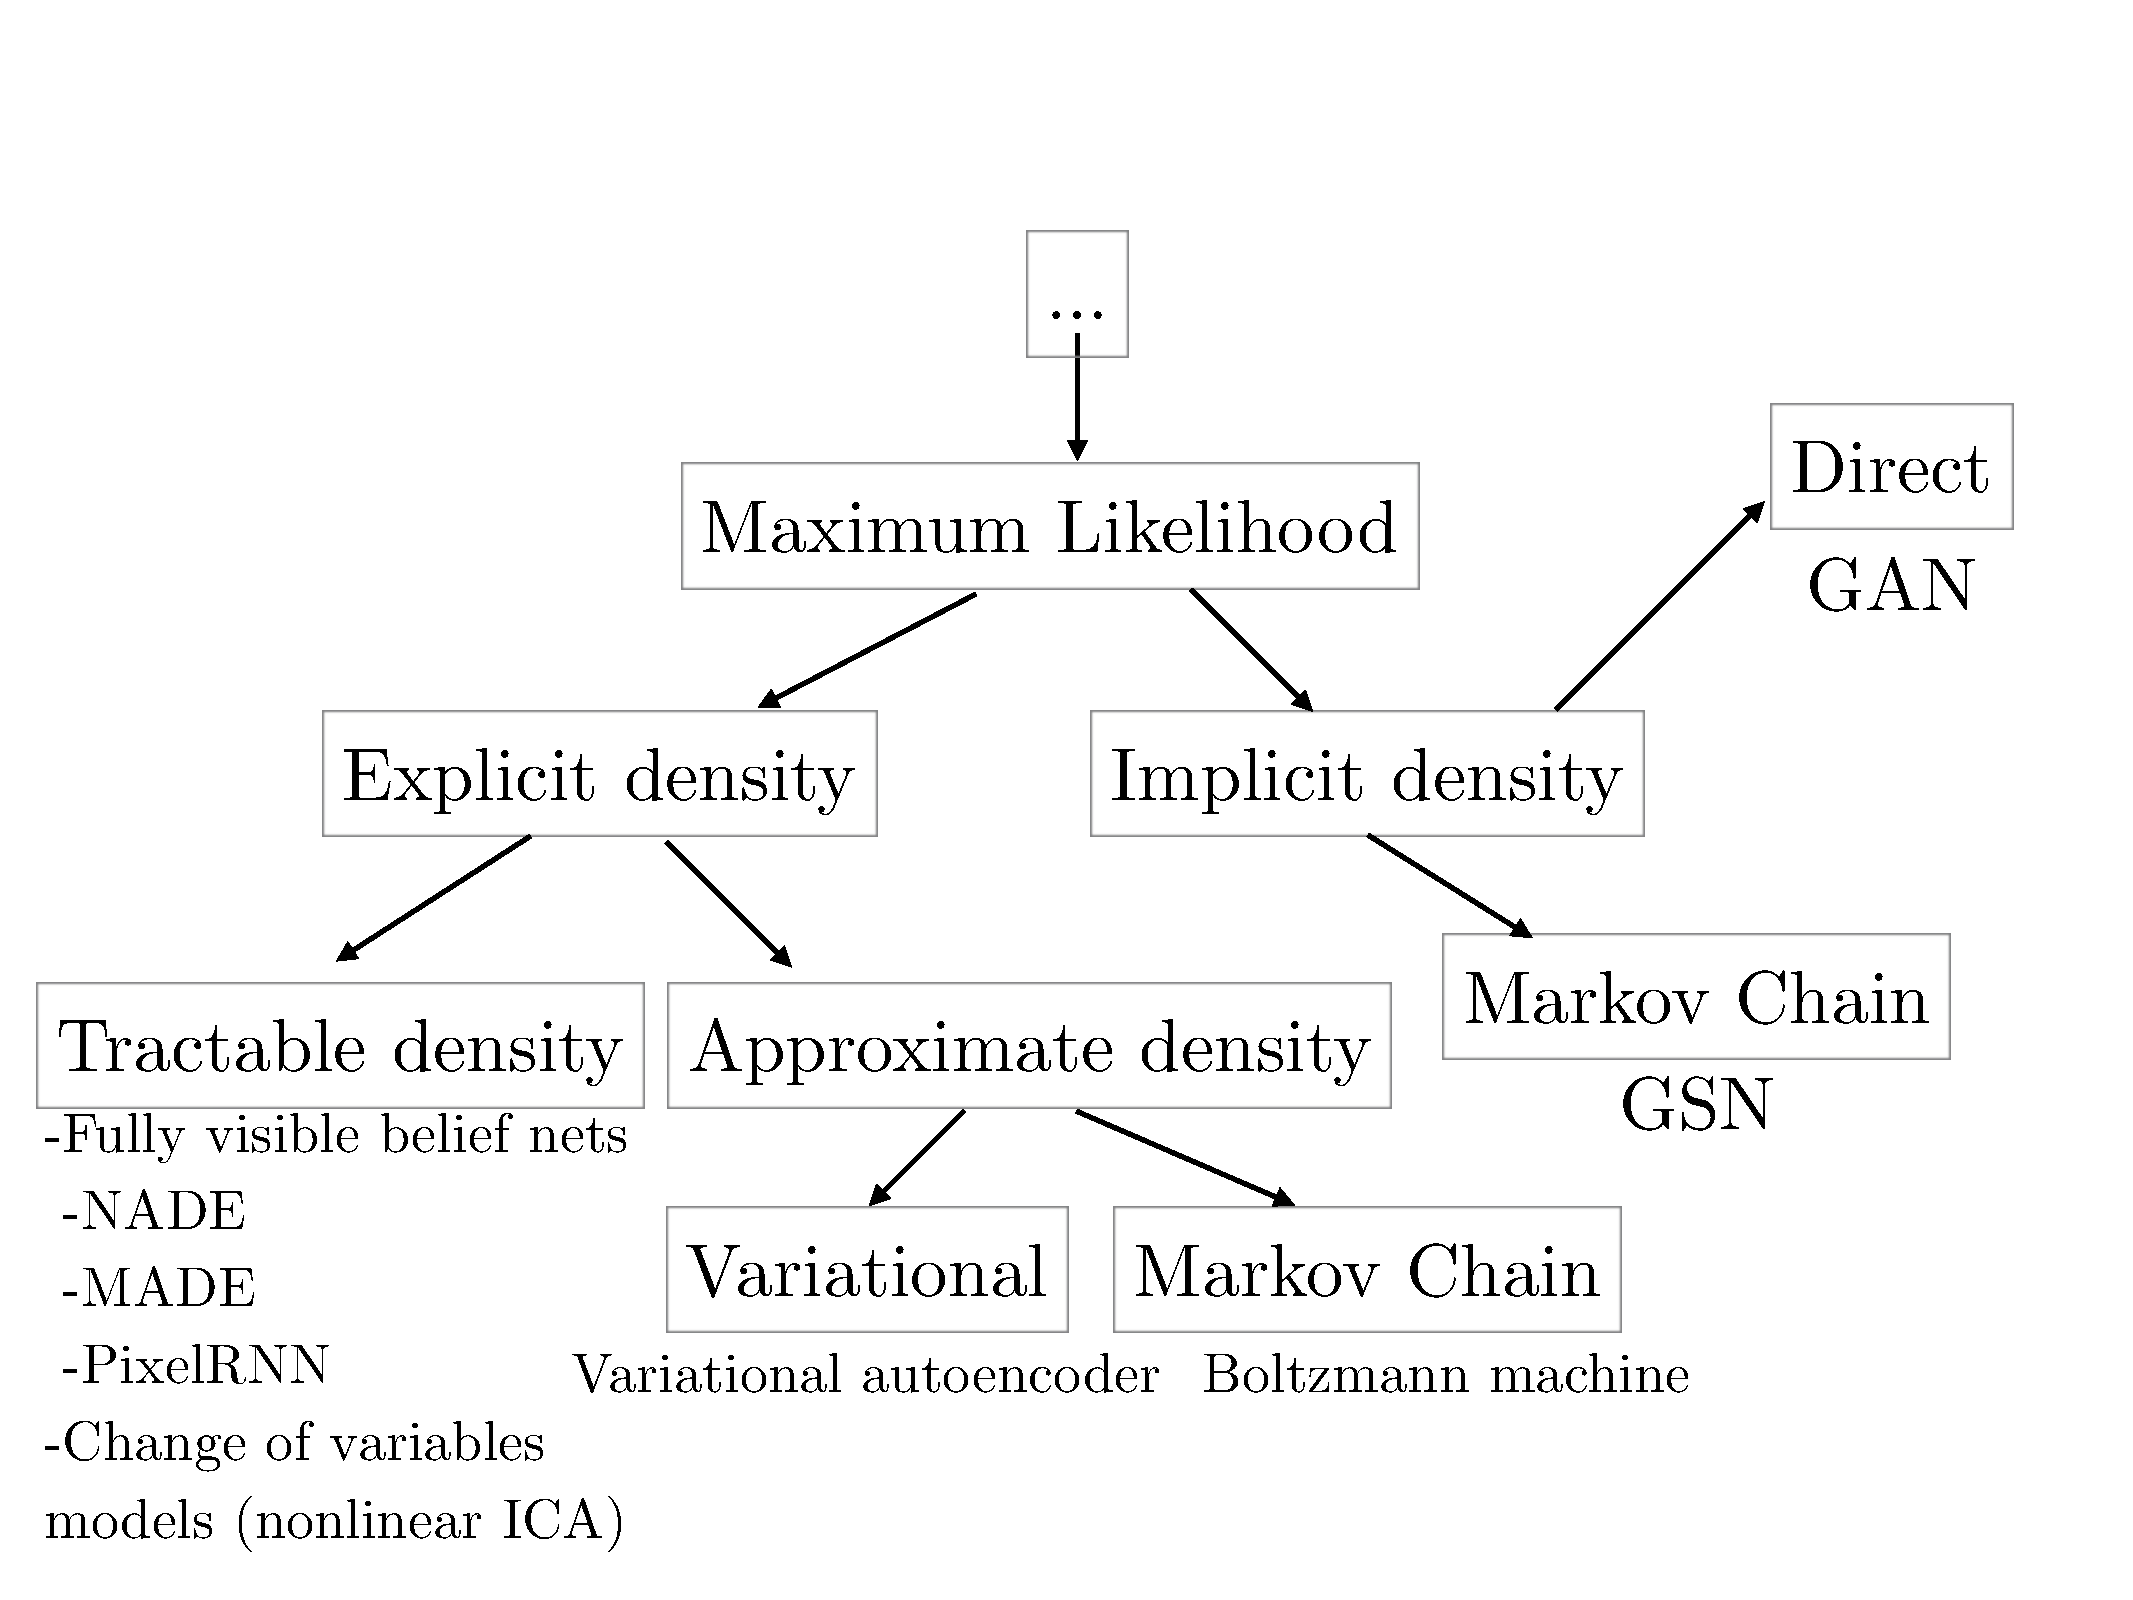
\includegraphics[width=\textwidth]{tree}
\caption{
Deep generative models that can learn via the principle of maximim likelihood
differ with respect to how they represent or approximate the likelihood.
On the left branch of this taxonomic tree, models construct an explicit density,
$\pmodel(\vx; \vtheta)$, and thus an explicit likelihood which can be maximized.
Among these explicit density models, the density may be computationally tractable,
or it may be intractable, meaning that to maximize the likelihood it is necessary
to make either variatioanl approximations or Monte
Carlo approximations (or both).
On the right branch of the tree, the model does not explicitly represent a
probability distribution over the space where the data lies.
Instead, the model provides some way of interacting less directly with this
probability distribution.
Typically the indirect means of interacting with the probability distribution is
the ability to draw samples from it.
Some of these implicit models that offer the ability to sample from the distribution
do so using a Markov Chain; the model defines a way to stochastically transform
an existing sample in order to obtain another sample from the same distribution.
Others are able to generate a sample in a single step, starting without any input.
While the models used for GANs can sometimes be constructed to define an explicit
density, the training algorithm for GANs makes use only of the model's ability to
generate samples.
GANs are thus trained using the strategy from the rightmost leaf of the tree:
using an implicit model that samples directly from the distribution represented
by the model.
}
\label{fig:tree}
\end{figure}

\subsection{Explicit density models}

In the left branch of the taxonomy shown in \figref{fig:tree} are models that define
an explicit density function $\pmodel(\vx ; \vtheta)$.
For these models, maxmimization of the likelihood is straightforward; we simply plug
the model's definition of the density function into the expression for the likelihood,
and follow the gradient uphill.

The main difficulty present in explicit density models is designing a model that can
capture all of the complexity of the data to be generated 
while still maintaining computational tractability.
There are two different strategies used to confront this challenge:
(1) careful construction of models whose structure guarantees their tractability,
as described in \secref{sec:explicit_tractable},
and (2) models that admit tractable approximations to the likelihood and its
gradients, as described in \secref{sec:approx}.

\subsubsection{Tractable explicit models}
\label{sec:explicit_tractable}

In the leftmost leaf of the taxonomic tree of \figref{fig:tree} are the models
that define an explicit density function that is computationally tractable.
There are currently two popular approaches to tractable explicit density models:
fully visible belief networks and nonlinear independent components analysis.

\paragraph{Fully visible belief networks}
{\em Fully visible belief networks} \citep{Frey96,Frey98} or FVBNs are models that use the chain
rule of probability to decompose a probability distribution over an $n$-dimensional vector $\vx$
into a product of one-dimensional probability distributions:
\[
\pmodel(\vx) = \prod_{i=1}^n \pmodel\left(\evx_i \mid \evx_1, \dots, \evx_{i-1} \right).
\]
FVBNs are, as of this writing, one of the three most popular
approaches to generative modeling, alongside GANs and variational autoencoders.
They form the basis for sophisticated generative models from DeepMind, such as
WaveNet \citep{aaron-wavenet-2016}. WaveNet is able to generate realistic human speech.
The main drawback of FVBNs is that samples must be generated
one entry at a time: first $\evx_1$, then $\evx_2$, etc., so the cost of generating
a sample is $O(n)$.
In modern FVBNs such as WaveNet, the distribution over each $\evx_i$ is computed by a deep
neural network, so each of these $n$ steps involves a nontrivial amount of computation.
Moreover, these steps cannot be parallelized.
WaveNet thus requires two minutes of computation time to generate one second of audio,
and cannot yet be used for interactive conversations.
GANs were designed to be able to generate all of $\vx$ in parallel, yielding greater
generation speed.

\paragraph{Nonlinear independent components analysis}
TODO

\subsubsection{Explicit models requiring approximation}
\label{sec:approx}

TODO
